\documentclass[conference]{IEEEtran}

\usepackage{pifont}
\usepackage{graphicx}
\usepackage{amsmath}
\usepackage{mybeamer}
\usepackage{draftwatermark}

\begin{document}

\title{Flow Specification of Cache Coherence Protocol in GEM5}

\maketitle


\begin{abstract}
This paper will go through a brief overview for the implemented instances of given GEM5 flow specifications. These flow specifications capture how messages are exchanged for different use cases. 
\end{abstract}

The flow specifications are implemented in a SoC model using GEM5. The architecture of this SoC model is shown in Fig.~\ref{SoC}. This SoC model consists of two ARM Cortex-A9 cores, each of which contains two separate 16KB data and instruction caches.  The caches are connected to a 1GB memory through a memory bus model.  .  

In this model, components communicate with each other by sending and receiving various request and response messages.  In order to observe and trace communications occurring inside this model during execution, monitors are attached to links connecting the components. These monitors record the messages flowing through the links they are attached to, and store them into output trace files. The recorded message is defined in the following format, (Src,Dest,Cmd), where Src and Dest refer to the source and destination components of messages, Cmd refers to the operations that the destination component should perform. 

\begin{figure} 
\centerline{
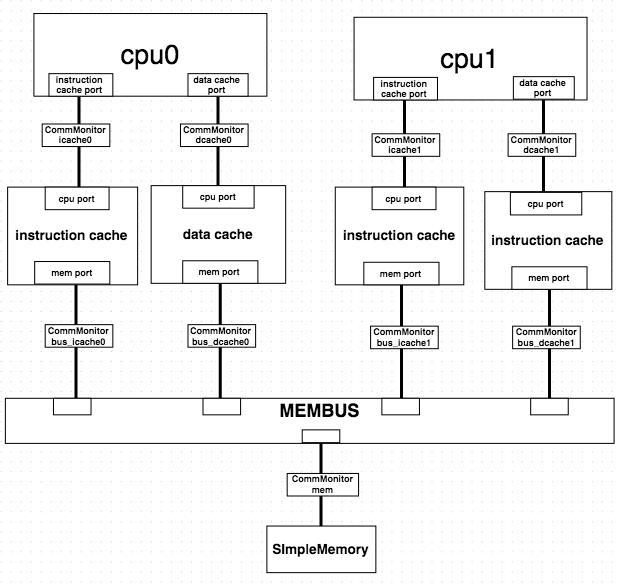
\includegraphics[width=3.3in]{figures/Fig4.png}}
\caption{SoC platform structure.}
\label{SoC}
\end{figure}


\section{write flow specification}

In this section, we will take CPU1 as an example to explain how write flow specification works in our SoC system.
 
Coherence protocol for write operation can be triggered by CPU1 initiating a memory write request to its data cache. Next, depends on whether the required data is included in cache1, and the status of requested data,  cache1 can generate three possible responses. 

First, the cache1 will send read exclusive request message msg2 to interconnect if data is not present in cache, as shown in Fig.~\ref{write3}.

 \begin{figure} 
 \centerline{
 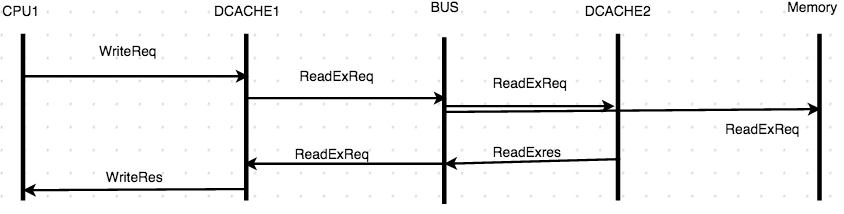
\includegraphics[width=4In]{figures/write3.png}}
 \caption{Flow sequence chart of write operation when requested data is not included in Dcache. ReadExRes can also be sent from Memory if Dcache2 doesn't have requested data. This sequence chart is symmetric for CPU2. }
 \label{write3}
 \end{figure}
 
 \begin{figure} 
 \centerline{
 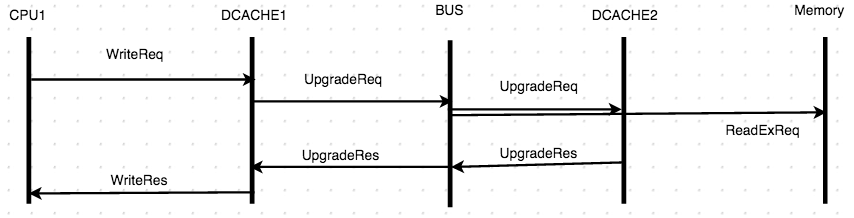
\includegraphics[width=4In]{figures/write2.png}}
 \caption{Flow sequence chart of write operation when requested data is shared by another component. UpgradeRes can also be sent from Memory if Dcache2 doesn't have requested data. This sequence chart is symmetric for CPU2. }
 \label{write2}
 \end{figure}

 \begin{figure} 
 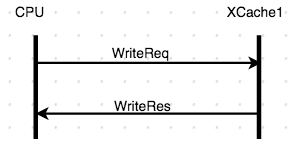
\includegraphics[width=1.9In]{figures/write1.png}
 \caption{Flow sequence chart of write operation when XCache has the exclusive right of requested data. XCache can be instruction cache or data cache. This sequence chart is symmetric for CPU2. }
 \label{write1}
 \end{figure}
 
Second, if the data is shared by CPU2, it will send upgrade request message msg16 to interconnect request disabling  CPU2's ownership of the data, as shown in Fig.~\ref{write2}. 

Last, if CPU1 has exclusive right of required data, ICache1 will perform the write operation and sent an response message msg15 to CPU1, as shown in Fig.~\ref{write1}.


\begin{figure} 
 \centerline{
 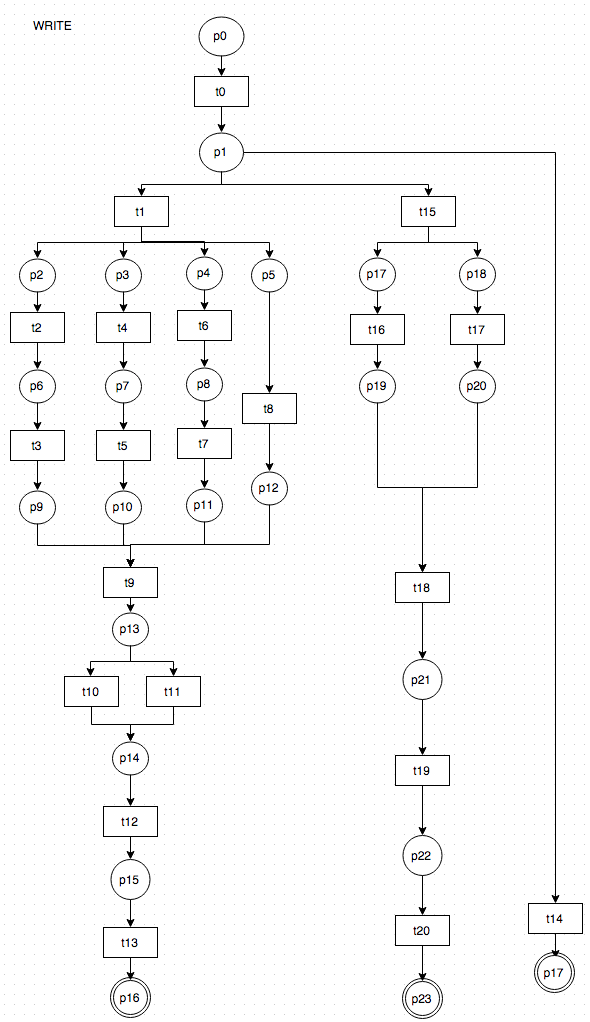
\includegraphics[width=3.4In]{figures/Fig5.png}}
 
 {\footnotesize
 \[
 \begin{array}{llll}
 msg_0: (&\mbox{ CPU1},&\mbox{writeReq},&\mbox{icache1   })\\       
 msg_1: (&\mbox{ dcache1},&\mbox{ readExreq },&\mbox{Bus     })\\        
 msg_2: (&\mbox{ Bus},&\mbox{ readExreq},&\mbox{ dcahce2 })\\  
 msg_3: (&\mbox{ dcache2},&\mbox{readExreq},&\mbox{cpu2         })\\   
 msg_4: (&\mbox{ Bus},&\mbox{ readExreq},&\mbox{ icahce2           })\\  
 msg_5: (&\mbox{ icache2},&\mbox{readExreq},&\mbox{cpu2 })\\  
 msg_6: (&\mbox{ Bus},&\mbox{ readExreq},&\mbox{ icahce1       })\\     
 msg_7: (&\mbox{ dcache1},&\mbox{readExreq},&\mbox{cpu1           })\\  
 msg_8: (&\mbox{ Bus},&\mbox{ readExreq},&\mbox{ Memory })\\  
 msg_9: (&\mbox{ true                                          })\\  
 msg_{10}: (&\mbox{ Memory},&\mbox{ readExres},&\mbox{ Bus})\\  
 msg_{11}: (&\mbox{ icache2},&\mbox{ readExres},&\mbox{ Bus })\\  
 msg_{12}: (&\mbox{ Bus},&\mbox{ readExres},&\mbox{ dcache1})\\  
 msg_{13}: (&\mbox{ icache1},&\mbox{ writeRes},&\mbox{ CPU1         })\\  
 msg_{14}: (&\mbox{ icache1},&\mbox{ writeRes},&\mbox{ CPU1 })\\  
 msg_{15}: (&\mbox{ dcache1},&\mbox{UpgradeReq},&\mbox{Bus})\\  
 msg_{16}: (&\mbox{ Bus},&\mbox{ UpgradeReq},&\mbox{ icahce2      })\\   
 msg_{17}: (&\mbox{ Bus},&\mbox{ UpgradeReq},&\mbox{ Memory })\\  
 msg_{18}: (&\mbox{ icache2},&\mbox{UpgradeRes},&\mbox{ Bus     })\\  
 msg_{19}: (&\mbox{ Bus},&\mbox{ UpgradeRes},&\mbox{ icache1      })\\  
 msg_{20}: (&\mbox{ icache1},&\mbox{ WriteRes},&\mbox{ CPU1 })\\  
 \end{array}
 \]}
 \caption{Flow specification of a cache coherent write operation initiated from CPU1. This flow is symmetric for CPU2. }
 \label{write-flow}
 \end{figure}


 Afterwards, interconnect will sent received request to all connected component (data cache and instruction cache of each CPU and memory). Once the interconnect obtains the response from either CPU2 or memory, it will generate a response message to cache1, cache1 will generate a write response message msg14 (or msg 21 ) to CPU1. These three flow sequence charts are implemented together in one flow specification in GEM5, as specified in Fig.~\ref{write-flow}.
 
 
 \section{read flow specification}
 In this section, we will also take CPU1 as an example to explain how read flow specification works in our SoC system.


 
 \begin{figure} 
 \centerline{
 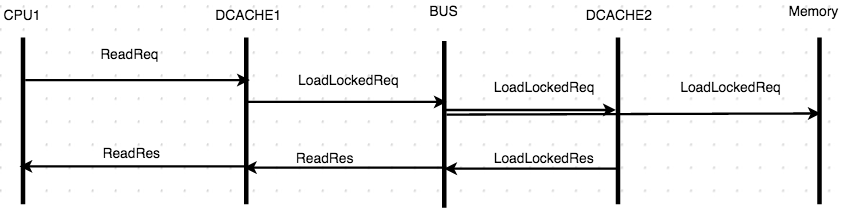
\includegraphics[width=3.9In]{figures/read3.png}}
 \caption{Flow sequence chart of read operation when requested data is shared by another component. LoadLockedRes can also be sent from Memory if Dcache2 doesn't have requested data. This sequence chart is symmetric for CPU2. }
 \label{read3}
 \end{figure}
 
 \begin{figure} 
 \centerline{
 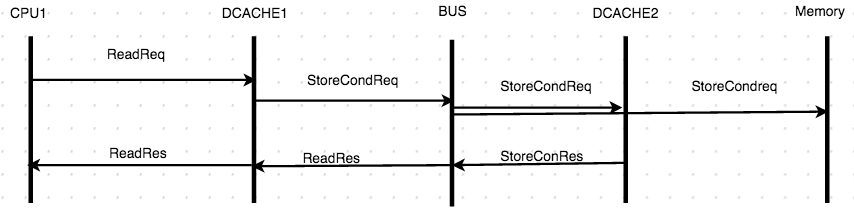
\includegraphics[width=3.9In]{figures/read2.png}}
 \caption{Flow sequence chart of read operation when requested data is not present. StoreCondRes can also be sent from Memory if Dcache2 doesn't have requested data. This sequence chart is symmetric for CPU2. }
 \label{read2}
 \end{figure}

 \begin{figure} 
 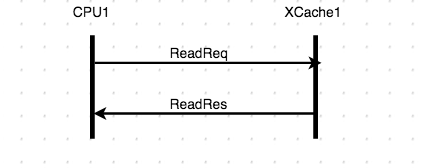
\includegraphics[width=2In]{figures/read1.png}
 \caption{Flow sequence chart of read operation when XCache has the exclusive right of requested data. XCache can be instruction cache or data cache. This sequence chart is symmetric for CPU2. }
 \label{read1}
 \end{figure}

 
Read coherence protocol can be triggered by CPU1 initiating a memory read request to its cache. Depending on whether the required data is included in its cache, the status of requested data,  and which cache the request is sent to, cache can generate three possible responses. 

First, for both instruction cache and data cache, if they have the exclusive right of requested data, they can generate a read response carrying the data back to CPU. Detailed flow sequence chart is displayed in Fig.~\ref{read1}.

Second, when ICache1 decide that the requested data is not present, it will issue an StoreCondReq to memory bus asking for data. 

Finally, if DCache1 has the data, but it's shared, it will issue an LoadLockedReq to memory bus requesting exclusive right of the data. Flow sequence charts for these two possibility are shown in Fig.\~ref{read1} and Fig.\~ref{read}.
 
Since instruction cache and data cache have different coherence protocol, there are two flow specifications for read operation generated by CPU1. The LPN specification as shown in Fig.~\ref{read-flow} captures the system flow where CPU1 initiate a memory read to instruction cache. And Fig.~\ref{read-dcache} specifies read operation to data cache from CPU1.


 \begin{figure} 
 \centerline{
 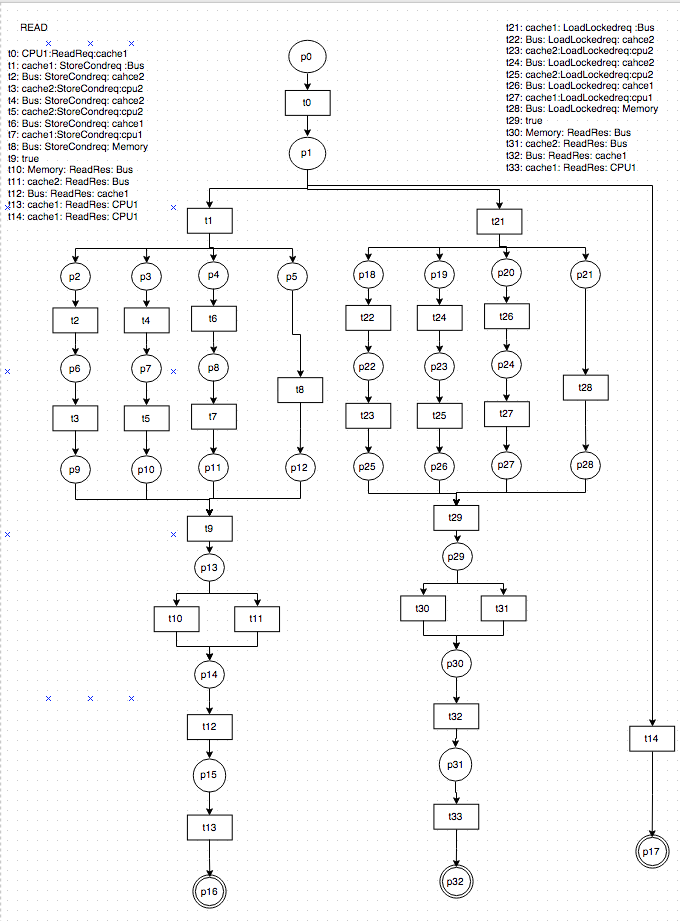
\includegraphics[width=3in]{figures/Fih6.png}}
 
 {\footnotesize
 \[
 \begin{array}{llll}
 msg0: (&\mbox{ CPU1},&\mbox{ReadReq},&\mbox{icache1  })\\                   
 msg1: (&\mbox{ dcache1},&\mbox{ StoreCondreq },&\mbox{Bus })\\           
 msg2: (&\mbox{ Bus},&\mbox{ StoreCondreq},&\mbox{ icahce2 })\\
 msg3: (&\mbox{ icache2},&\mbox{StoreCondreq},&\mbox{cpu2       })\\      
 msg4: (&\mbox{ Bus},&\mbox{ StoreCondreq},&\mbox{ dcahce2           })\\ 
 msg5: (&\mbox{ dcache2},&\mbox{StoreCondreq},&\mbox{cpu2 })\\
 msg6: (&\mbox{ Bus},&\mbox{ StoreCondreq},&\mbox{ dcahce1     })\\       
 msg7: (&\mbox{ icache1},&\mbox{StoreCondreq},&\mbox{cpu1           })\\ 
 msg8: (&\mbox{ Bus},&\mbox{ StoreCondreq},&\mbox{ Memory })\\
 msg9: (&\mbox{ true                                        })\\
 msg10: (&\mbox{ Memory},&\mbox{ ReadRes},&\mbox{ Bus            })\\    
 msg11: (&\mbox{ icache2},&\mbox{ ReadRes},&\mbox{ Bus })\\
 msg12: (&\mbox{ Bus},&\mbox{ ReadRes},&\mbox{ dcache1      })\\            
 msg13: (&\mbox{ icache1},&\mbox{ ReadRes},&\mbox{ CPU1          })\\  
 msg14: (&\mbox{ icache1},&\mbox{ ReadRes},&\mbox{ CPU1 })\\
 \end{array}
 \]}
 \caption{Flow specification of a cache coherent read operation initiated from CPU1 to instruction cache.This flow is symmetric for CPU2. }
 \label{read-flow}
 
 \end{figure}
 
 

 \begin{figure} 
 \centerline{
 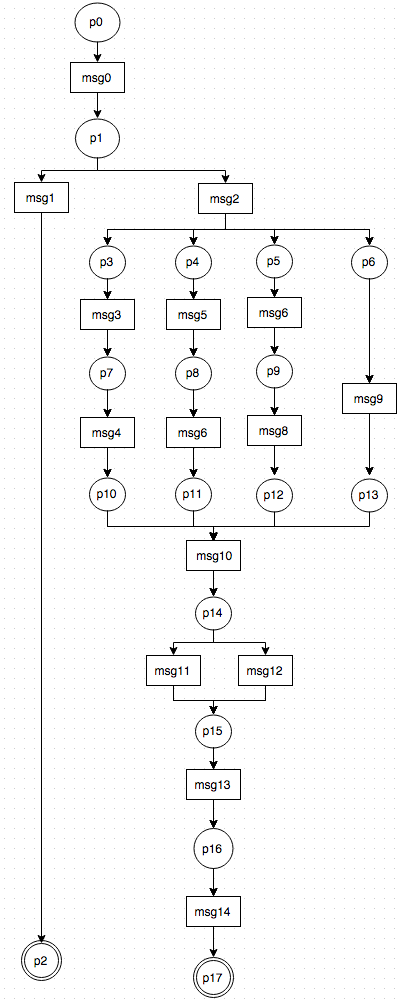
\includegraphics[width=3in]{figures/readDcache.png}}
 
 {\footnotesize
 \[
 \begin{array}{llll}
 msg0: (&\mbox{ CPU1},&\mbox{ReadReq},&\mbox{dcache1  })\\                   
 msg1: (&\mbox{ dcache1},&\mbox{ ReadRes},&\mbox{ CPU1 })\\
 msg2: (&\mbox{ icache1},&\mbox{ LoadLockedreq },&\mbox{Bus })\\     
 msg3: (&\mbox{ Bus},&\mbox{ LoadLockedreq},&\mbox{ dcahce2     })\\
 msg4: (&\mbox{ dcache2},&\mbox{LoadLockedreq},&\mbox{cpu2 })\\
 msg5: (&\mbox{ Bus},&\mbox{ LoadLockedreq},&\mbox{ icahce2     })\\ 
 msg6: (&\mbox{ icache2},&\mbox{LoadLockedreq},&\mbox{cpu2     })\\
 msg7: (&\mbox{ Bus},&\mbox{ LoadLockedreq},&\mbox{ dcahce1 })\\
 msg8: (&\mbox{ icache1},&\mbox{LoadLockedreq},&\mbox{cpu1       })\\
 msg9: (&\mbox{ Bus},&\mbox{ LoadLockedreq},&\mbox{ Memory     })\\
 msg10: (&\mbox{ true })\\
 msg11: (&\mbox{ Memory},&\mbox{ ReadRes},&\mbox{ Bus       })\\     
 msg12: (&\mbox{ icache2},&\mbox{ ReadRes},&\mbox{ Bus    })\\
 msg13: (&\mbox{ Bus},&\mbox{ ReadRes},&\mbox{ icache1 })\\
 msg14: (&\mbox{ dcache1},&\mbox{ ReadRes},&\mbox{ CPU1 })\\
 \end{array}
 \]}
 \caption{Flow specification of a cache coherent read operation initiated from CPU1 to  data cache. This flow is symmetric for CPU2. }
 \label{read-dcache}
 
 \end{figure}

\section{failed read specification}

\begin{figure} 
 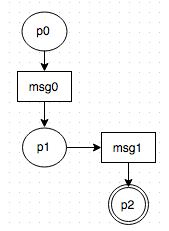
\includegraphics[width=1.5in]{figures/storeFail.png}
 
 {\footnotesize
 \[
 \begin{array}{llll}
 msg0: (&\mbox{ CPU1},&\mbox{StoreCondFailedReq},&\mbox{ICache1})\\                   
 msg1: (&\mbox{ ICache1},&\mbox{ StoreCondFailedRes},&\mbox{ CPU1 })\\
 \end{array}
 \]}
 \caption{Flow specification of failed read. This flow is symmetric for CPU2. }
 \label{storefail}
 
 \end{figure}
Another flow implemented in GEM5 is when CPU initiate a store failed request to instruction cache, with a simple store failed response from instruction cache. Detailed flow specification is specified in Fig.~\ref{storefail}

This three specifications are also symmetric for CPU2.
\end{document}
